\documentclass[a4paper, 11pt]{article}
\topmargin -1.2cm \textheight 22cm \evensidemargin 0cm
\oddsidemargin 0cm \textwidth 15.23cm \flushbottom
\usepackage{amsmath}
\usepackage{graphicx}
\usepackage{color}
\usepackage{amsfonts}
\usepackage{portland}
\usepackage{lscape}
\newtheorem{theorem}{Theorem}[section]
\newtheorem{dfn}{Definition}[section]
\newtheorem{note}{Remark}[section]
\numberwithin{equation}{section}
\linespread{1.2}\Large
\begin{document}
\begin{titlepage}
	\centering
	
\includegraphics[width=0.15\textwidth]{itu.jpg} \par\vspace{1cm}
	{\scshape\LARGE Istanbul Technical University \par}
	\vspace{1cm}
	{\scshape\Large Final year project\par}
	\vspace{1.5cm}
	{\huge\bfseries Estimation of Burr XII Distribution Based on Generalized Order Statistics\par}
	\vspace{2cm}
	{\Large\itshape Ismet Artuc\par}
	\vfill
	supervised by\par
	Assoc. Dr. Mustafa \textsc{NADAR}
	\vfill

% Bottom of the page
	{\large \today\par}
\end{titlepage}
\title{\bf Estimation of Burr XII distribution based on generalized order statistics}
\author{ Ismet ARTUC \\
\small {Department of Mathematical Engineering, Istanbul  Technical University, Istanbul, Turkey.} \\ }
\date{}
\maketitle
\tableofcontents
\newpage
\begin{abstract}
The ordered random variables play important roles in the theory and practice of statistics. They possess significant statistical properties. Over the last few decades, many articles on various topics of ordered statistical data have appeared. It was a special interest to coordinate and edit an interesting research problem based on material contributed by several important researchers from all over the world. In this study the estimation of parameters with different methods using the $ k^{ht}$ record values from Burr XII distribution will be discussed and based on different estimation hazard function will be obtained.
\end{abstract}

\section{Order Statistics and Record Values}
 Order statistics and record values appear in many statistical applications and are widely used in statistical modeling and inference. A form of the joint distribution of $ n $ ordered random variables is presented that enables a unified approach to a variety of models of ordered random variables, e.g. order statistics and record values. Generalized order statistics, provide a suitable approach to explain similarities and analogies in the two models and to generalize related results. 
 
Kamps (1995) introduced the concept of generalized order statistics (gos) as a unified approach to order statistics, record values, and sequential order statistics. The gos are defined using quantile transformation based on the distribution function F.

Let $X(1, n, m,k),\ldots, X(r, n,m,k), k > 1 $, m is a real number, be gos based on absolutely continuous distribution function F with density function f. The joint density function of the above quantities is given by
\begin{equation}
f^{X(1,n,m,k), \ldots, X(r,m,n,k)}(x_{1},....,x_{r})
= C_{r-1}\big( \prod\limits_{i=1}^{n}  [1-F(x_i)]^{m} f(x_i) [1-F(x_r)]^{&_r-1}f(x_r)\big),\\
\end{equation}
\begin{equation*}
F^{-1}(0+)<x_1 \leq....\leq x_r<F^{-1}(1),

\noindent \text{where}\\
&\gamma_r=k+(n-r)(m+1)>0,~~~~
C_{r-1}={\overset{r}{\underset{j=1}{\prod}&\gamma_j}~, ~~~~~~ r=1,2,\ldots, n ,~~~~ \gamma_n=k.
%
\end{equation*}

\noindent with $n \in{N}  , k > 0}$  and $ m \in{R}.}$ For more details of gos, see Kamps (1995). In the case $m = 0$ and $k = 1$, $X(r, n, m, k)$ reduces to the ordinary $ r^{th} $ order statistics and (1.1) is the joint pdf of r ordinary order statistics, $X_{1:n} ≤ X_{2:n} ≤ ··· ≤ X_{r:n}$. For various distributional properties of ordinary order statistics, see David (1981) and Arnold et al. (1992).
 If $m = −1$ and $k = 1$, then (1.3) is the joint pdf of r upper record values. For some distributional properties of record values, see Ahsanullah (1995) and Arnold et al. (1998). \\
 
The definition of random  $ k^{ht}$  record  can  be  shown  as  below. 
Let $ X_1, X_2, . . . $ be a sequence of independent and identically distributed (i.i.d.) random variables with continuous distribution function  $ F(x) = P (X_1 \leq x)$. Denote by  $X{(1,n)} \leq . . . \leq X{(n,n)}$, $n$ the order statistics of  $ X_1, . . . , X_n.$ For a fixed integer  $k \geq 1,$ we define the corresponding  $k^{ht}$record times, ${L(n, k), n \geq 1}$, and  $k^{ht} $ record values ,  
${X{(n, k)}, n \geq 1},$ by setting
$  L(1, k) = k,	L(n + 1, k) = min\{j > L(n, k) : X_{j} > X_{j-k,j-1}\}$ for $n \geq 1 $, and
$ X_{(n, k)} = X_{L(n,k)−k+1,L(n,k)} $	for	  $n \geq 1.$\\
Let N be a positive integer-valued random variable which is independent of the $ X_{i}. $ The random variables X(N, k) are called the random $k^{th} $ record.

\section{Hazard Function}

Now we will discuss the hazard function. Hazard function is generally used when calculating the age of an electronic device or any material. The failure rate of a system usually depends on time, with the rate varying over the life cycle of the system. For example, an automobile's failure rate in its fifth year of service may be many times greater than its failure rate during its first year of service.
Many probability distributions can be used to model the failure distribution.

\section{Burr XII Function}

Burr distribution was first introduced by Burr (1942) as a two-parameter family. An additional scale parameter was introduced by Tadikamalla (1980). The Bayesian estimation for the two parameters of some lifetime distributions,including exponential, Weibull, Pareto and Burr Type XII, based on upper record values was considered by Ahmadi and Doostparast (2006). Estimation and prediction of the Burr type XII distribution based on record values and interrecord times was studied by Mustafa Nadar & Fatih Kızılaslan (2015). The Burr distribution can fit a wide range of empirical data. Different values of its parameters cover a broad set of skewness and kurtosis. Hence, it is used in various fields such as finance, hydrology, and reliability to model a variety of data types. Examples of data modeled by the Burr distribution are household income, crop prices, insurance risk, travel time, flood levels, and failure data.

The two parameter Burr type XII distribution which is denoted by Burr XII $(\alpha, \beta)$ has the following probability density function $(pdf)$ of the form
\begin{equation}
f(x; \alpha, \beta)=\alpha \beta ~x^{\alpha-1}(1+x^{\alpha})^{-(\beta+1)},~~x>0,~~\alpha, \beta>0
\label{eq:ge1}
\end{equation}
and a cumulative distribution function $(cdf)$
\begin{equation} 
F(x; \alpha, \beta)=1-(1+x^{\alpha})^{-\beta},~~x>0,~~\alpha, \beta>0
\label{eq:ge2}
\end{equation}
%
Hazard functions of Burr type XII distribution is,
\begin{equation}
h(x|\alpha,\beta)=\frac{\alpha\beta x^{\alpha-1}}{1+x^{\alpha}}
\end{equation}
\\
 Distribution properties of gos from a uniform distribution are given by Ahsanullah (1996). He obtained the minimum variance linear unbiased estimators of the parameters of the two parameters of uniform distribution based on the first m gos Kamps (1996) characterized the uniform distribution based on distribution properties of subranges of gos. Kamps and Gather (1997) characterized the exponential distributions by distributional properties of gos Cramer and Kamps (1996, 1998, 2001) studied some estimation problems with different sequential k-out-of-n systems. Ahsanullah (2000) gave some distributional properties of the gos from the two parameter exponential distribution. He also obtained the minimum variance linear unbiased estimators of the two parameters and characterized the exponential distribution based on gos. Cramer and Kamps (2000) derived relations for expectations of functions of gos from a class of distributions which includes the exponential, uniform and Pareto. Habibullah and Ahsanullah (2000) obtained estimates for the parameters of the Pareto distribution based on gos. Kamps and Cramer (2001) studied some distribution properties of the gos from the Pareto, power and Weibull distributions. Jaheen (2002) considered the prediction of future gos from a general class of distributions which includes the Weibull, compound Weibull, Burr type XII, Pareto, beta, and Gompertz by using Bayesian  two-sample  prediction technique.
\section{Maximum likelihood estimation}
The log likelihood function $l(\alpha, \beta|\mathbf{x})=\log L(\alpha, \beta|\mathbf{x})$, dropping terms that do not involve $\alpha$ and $\beta$, is 
\begin{equation*}
l(\alpha, \beta|\mathbf{X=x})=nln\alpha+nln\beta+(\alpha-1)\sum_{i=1}^{n-1}ln x_{i}-(m\beta+\beta+1)\sum_{i=1}^{n-1}ln(1+x_{i}^{\alpha})
\end{equation*}
\begin{equation}
+(\alpha-1)lnx_{n}-(k\beta+1)ln(1+x_{n}^{\alpha}).
\end{equation}
We assume that the parameters $\alpha$ and $\beta$ are unknown. To obtain the normal equations for the unknown parameters, we differentiate (4.1) partially with respect to $\alpha$ and $\beta$ and equate to zero, the resulting equations are 
\begin{equation}
0=\frac{\partial l(\alpha, \beta|\mathbf{x})}{\partial \alpha}=\frac{n}{\alpha}+\sum_{i=1}^{n}ln x_{i}-\sum_{i=1}^{n}x_{i}^{\alpha}\upsilon_{i}-\beta\left[(1+m)\sum_{i=1}^{n-1}x_{i}^{\alpha}\upsilon_{i}+k x_{n}^{\alpha}\upsilon_{n}\right],
\label{alfa_mle}
\end{equation}

and
\begin{equation}
0=\frac{\partial l(\alpha, \beta|\mathbf{x})}{\partial \beta}=\frac{n}{\beta}+(m+1)\sum_{i=1}^{n-1}ln x_{i}^{\alpha}\delta_{i}+k~ln x_{n}^{\alpha}\delta_{n},
\label{beta_mle}
\end{equation}
where
$\delta_{i}=\frac{x_{i}^{\alpha}}{1+x_{i}^{\alpha}}$ and $\upsilon_{i}=\frac{ln x_{i}}{1+x_{i}^{\alpha}}$.\\The solutions of the above equations are the maximum likelihood estimators of the Burr XII $(\alpha, \beta)$ parameters $\alpha$  and $\beta$, denoted  $\hat{\alpha}_{MLE}$  and $\hat{\beta}_{MLE}$, respectively. As the equations expressed in (23) and (24) cannot be solved analytically, one must use a numerical procedure to solve them.

\section{Bayesian  estimation}
In this section we consider Bayesian estimation of the unknown parameters of the Burr XII $(\alpha, \beta)$ under squared error loss function $(SEL)$. It is assumed that  $\alpha$  and $\beta$   has the independent gamma prior distributions with probability density functions
\begin{equation}
h(\alpha)\propto \alpha^{a-1}e^{-b\alpha},~~\alpha>0
\end{equation}
and
\begin{equation}
h(\beta)\propto \beta^{c-1}e^{-d\beta},~~\beta>0.
\end{equation}
The hyper-parameters $a$, $b$, $c$, and $d$ are known and non-negative. If both the parameters $\alpha$  and $\beta$  are unknown, joint conjugate priors do not exist. It is not unreasonable to assume independent gamma priors on the shape and scale parameters for a two-parameter  Burr XII $(\alpha, \beta)$, because gamma distributions are very flexible, and the Jeffrey's (non-informative) prior, introduced by Jeffrey (1946) is a special case of this. The joint prior distribution in this case is
\begin{equation}
h(\alpha, \beta)\propto \alpha^{a-1} e^{-b\alpha} \beta^{c-1} e^{-d\beta},~~\alpha,~\beta>0.
\end{equation}
Combining (27) with  (21) and using Bayes theorem, the joint posterior distribution is derived as
\begin{equation}
\pi(\alpha, \beta|\mathbf{x})\propto\alpha^{n+a-1} \beta^{n+c-1}e^{-b\alpha-d\beta}\left(\prod_{i=1}^{n-1}\frac{x_{i}^{\alpha-1}}{(1+x_{i}^{\alpha})^{m\beta+\beta+1}}\right)\frac{x_{n}^{\alpha-1}}{(1+x_{n}^{\alpha})^{k\beta+1}}.
\label{joint_post}
\end{equation}

 Bayes estimator of any function of $\alpha $ and $\beta $, say $g(\alpha
,\beta )$ under the SE loss function is its posterior mean. Therefore, the
Bayes estimator of $g(\alpha ,\beta )$ under the SE loss function is%
\begin{equation}
\widehat{g}_{BS}=E_{\left. \alpha ,\beta \right\vert \mathbf{r,k}}(g(\alpha
,\beta ))=\frac{\int_{0}^{\infty }\int_{0}^{\infty }g(\alpha ,\beta
)L(\alpha ,\beta ;\mathbf{r,k})\pi (\alpha ,\beta )d\alpha d\beta }{%
\int_{0}^{\infty }\int_{0}^{\infty }L(\alpha ,\beta ;\mathbf{r,k})\pi
(\alpha ,\beta )d\alpha d\beta }.  \label{eq17}
\end{equation}%
It is not possible to compute Equation (\ref{eq17}) analytically. Lindley's approximation is suggested here to approximate Equation (\ref{eq17}).

\paragraph{Lindley's approximation}

Lindley (1980) proposed a method to approximate the ratio of integrals such
as Equation (\ref{eq17}). For the two parameter case $(\alpha ,\beta )$, the Lindley's approximation can be
written as 
\begin{equation}
\widehat{g}_{Lind}(\alpha ,\beta )=g(\widetilde{\alpha },\widetilde{\beta })+%
\frac{1}{2}\left[ B+Q_{30}B_{12}+Q_{21}C_{12}+Q_{12}C_{21}+Q_{03}B_{21}%
\right] ,  \label{eq18}
\end{equation}%
where $B=\sum_{i=1}^{2}\sum_{j=1}^{2}g_{ij}\tau _{ij}$, $Q_{ij}=\partial
^{i+j}Q/\partial ^{i}\alpha \partial ^{j}\beta $, for $i,j=0,1,2,3$ and $%
i+j=3$, $g_{1}=\partial g/\partial \alpha $, $g_{2}=\partial g/\partial
\beta ,$ $g_{ij}=\partial ^{2}g/\partial \alpha ^{i}\partial \beta ^{j}$ for 
$i,j=1,2$ and $B_{ij}=(g_{i}\tau _{ii}+g_{j}\tau _{ij})\tau _{ii}$ and $%
C_{ij}=3g_{i}\tau _{ii}\tau _{ij}+g_{j}(\tau _{ii}\tau _{ij}+2\tau
_{ij}^{2}) $ for $i\neq j$, where $\tau _{ij}$ is the $(i,j)$th element in
the inverse of the matrix $Q^{\ast }=(-Q_{ij}^{\ast }),$ $i,j=1,2$ such that 
$Q_{ij}^{\ast }=\partial ^{2}Q/\partial \alpha ^{i}\partial \beta ^{j}$, $Q$
is the logarithm of the posterior density function, dropping terms that do not involve $\alpha$ and $\beta$,
$(\widetilde{\alpha },%
\widetilde{\beta })$ is the joint posterior mode of $Q$ and $\widehat{g}%
_{Lind}(\alpha ,\beta )$ is evaluated at $(\widetilde{\alpha },\widetilde{%
\beta })$.

For our case, we have from Equation (28) %
\begin{equation}
\begin{aligned}
Q=&(n+a-1)\ln \alpha +(n+c-1)\ln \beta -(\alpha-1)\underset{i=1}{\overset{n}{\sum }}\ln x_{i}- \underset{i=1}{\overset{n}{\sum }}\ln (1+x_{i}) \\
-&\beta \big[ d+(m+1)\underset{i=1}{\overset{n-1}{\sum }}\ln (1+x_{i})^{\alpha} +k \ln(1+x_{n}^{\alpha}) \big]-b \alpha 
% \label{eq19}
\end{aligned}
\end{equation}%

The joint posterior mode is obtained from system equations $\partial Q/\partial
\alpha =0$ and $\partial Q/\partial \beta =0$. Therefore, 
\begin{equation}
\widetilde{\beta }=\frac{n+c-1}{d+\big [(m+1)\underset{i=1}{\overset{n-1}{\sum }}\ln (1+x_{i}^{\widetilde{\alpha }}) +k \ln(1+x_n^{\widetilde{\alpha }}) \big]},
% \label{eq20}
\end{equation}%
and $\widetilde{\alpha }$ is the solution of the following nonlinear equation%
\begin{equation}
\frac{n+a-1}{\alpha }-\underset{i=1}{\overset{n}{\sum }}\frac{\ln(x_i)}{1+x_i^\alpha}-\beta \big[ (m+1) \underset{i=1}{\overset{n-1}{\sum }} \frac{x_i^\alpha \ln(x_i)}{1+x_i^\alpha} 
+\frac{k x_n^\alpha \ln(x_n)}{1+x_n^\alpha} \big] -b = 0
% \label{eq21}
\end{equation}%
It can be solved by using the same procedure in Equations (\ref{alfa_mle}) and (%
\ref{beta_mle}). The elements of the $Q^{\ast }$ are given by 
\begin{equation}
Q_{11}^{\ast }=-\frac{(n+a-1)}{\alpha ^{2}}-\underset{i=1}{\overset{n}{%
\sum }} x_i^\alpha \big(  \frac{\ln (x_i)}{1+x_i^\alpha }\big)^2-\beta (m+1)\underset{i=1}{\overset{n-1}{\sum }} x_i^\alpha \big( \frac{\ln (x_i)}{1+x_i^\alpha}\big )^2-
\beta k x_n^\alpha \big( \frac{\ln (x_n)}{1+x_n^\alpha} \big)^2
\label{Q11}
\end{equation}%

\begin{equation}
Q_{12}^{\ast }=Q_{21}^ {\ast}=- (m+1)\underset{i=1}{\overset{n-1}{\sum }} x_i^\alpha \frac{\ln (x_i)}{1+x_i^\alpha}- k x_n^\alpha \frac{\ln (x_n)}{1+x_n^\alpha}
\label{Q21}
\end{equation}%


\begin{equation}
Q_{22}^{\ast }=-\frac{(n+c-1)}{\beta ^{2}}
\label{Q22}
\end{equation}%



and $\tau _{ij},$ $i,j=1,2$ are obtained by using Equation (\ref{Q11})-(\ref{Q22}).
Moreover, we have%
\begin{equation*}
Q_{12}=0,\text{ }Q_{21}=- (m+1)\underset{i=1}{\overset{n-1}{\sum }} x_i^\alpha (\frac{\ln (x_i)}{1+x_i^\alpha})^2- k x_n^\alpha (\frac{\ln (x_n)}{1+x_n^\alpha})^2, 
\text{ }Q_{03}=\frac{2\left( n+c-1)\right) }{\beta^3 },
\end{equation*}%

\begin{equation*}
\begin{aligned}
Q_{30}=&\frac{2\left( n+a-1\right) }{\alpha ^{3}}-\underset{i=1}{%
\overset{n}{\sum }} x_i^\alpha (1-x_i^\alpha )\left( \frac{\ln x_{i}}{1+x_{i}^{\alpha }}\right) ^{3}-
\beta(m+1)\underset{i=1}{\overset{n-1}{\sum }} x_i^\alpha(1-x_i^\alpha )\left( \frac{\ln x_{i}}{1+x_{i}^{\alpha }}\right) ^{3} \\
-&\beta k X_n^\alpha(1-x_n^\alpha)\left( \frac{\ln x_{n}}{1+x_{n}^{\alpha }}\right) ^{3}
\end{equation*}%

Therefore, the approximate Bayes estimators of $\alpha $ and $\beta $ under
the SE  loss function is obtained as 
\begin{eqnarray}
\widehat{\alpha }_{Lind} &=&\widetilde{\alpha }+\frac{1}{2}\left[
Q_{30}\tau _{11}^{2}+3Q_{21}\tau _{11}\tau _{12}+Q_{03}\tau _{21}\tau _{22}%
\right] ,  \label{eq23} \\
\widehat{\beta }_{Lind} &=&\widetilde{\beta }+\frac{1}{2}\left[
Q_{30}\tau _{11}\tau _{12}+Q_{21}(\tau _{11}\tau _{22}+2\tau
_{12}^{2})+Q_{03}\tau _{22}^{2}\right] .
\label{eq24}
\end{eqnarray}%
Notice that all approximate Bayes estimators are evaluated at $(\widetilde{%
\alpha },\widetilde{\beta })$.


\section{Simulation study}
In this section, we present some numerical results to compare the performances of the estimators of $\alpha $ and $\beta $ for $k=1$ (ordinary record case) and $k=2$ (second order case) which are obtained 
using different methods for different sample sizes described in the preceding sections. The performances of the point estimators are compared  using estimated risks (ERs). The estimated risk (ER) of $\theta $, when $\theta $ is estimated by $
\begin{equation*}
ER(\theta )=\frac{1}{N}\underset{i=1}{\overset{N}{\sum }}\left( \widehat{%
\theta }_{i}-\theta _{i}\right) ^{2}, 
\end{equation*}% 
under the SE loss function.  Moreover, the hazard functions for $k=1$ (ordinary record case) and $k=2$ (second order case) are obtained using different methods for different sample sizes described in the preceding sections.

All of the computations are performed by using Matlab R2014a. All the results are based on 1000 replications.

In the simulation, the populations are generated for $(\alpha ,\beta
)=(3.1007, 3.4367)$ and for different sample sizes $n=10,$ $15$. In case of
Bayesian estimation, the hyperparameters values are taken as  $\alpha $ is $(a_{1},b_{1})=(1.0502,0.3387)$
and for $\beta $ is $(c,d)=(1.4826,0.4314).$

It is observed that the average ERs for the estimates of $\alpha $ and $%
\beta $ decrease as the sample size increases in all cases, as expected. The
Bayes estimates of $\alpha $ and $\beta $ under the SE loss function have
smaller ER than that of MLEs. Furthermore, from the graphs in general, we observed that the hazard function by using lindley approximation is closer to the true valued hazard function when compared to the MLE case.  
%%%%%%%%%%%%%%%%%%%%
\section{Tables}
The estimated parameter values for MLE, ordinary records and 2nd record using different methods of estimation are presented below.
\bigskip
%\begin{landscape}

Table 1. Estimates of $\alpha$, $\beta$ for the ordinary record values by using different methods when the Prior are $(a, b )= (1.0502, 0.3387)$ and $(c, d) =(1.4826, 0.4314)$

\begin{tabular}{lcccl}
\hline \hline
& & & & & \multicolumn{1}{l}{} \\
$n$ & $\alpha $ & & MLE & \begin{tabular}[b]{c} Bayes estimates \\Lindley  \end{tabular} \\ \hline
10 & 3.1007 & &  3.4201 & 3.3982 &  \\ 
& & ER & 1.4114 & 0.8115&  \\

& $\beta $ &   &    \\ \hline
& 3.4367 & &  3.8663  & 3.8877 &  \\ 
& & ER & 2.7787 & 1.3692   \\

$n$ & $\alpha $ & & MLE & Lindley  \\ \hline
15 & 3.1007 & & 3.3695 & 3.3933 &  \\ 
& & ER & 1.3353 &  0.7476 &  \\

& $\beta $ &   &    \\ \hline
&3.4367 & & 3.8085 & 3.8728 &  \\ 
& & ER & 2.3638 &  1.2154 &  \\ \hline
\end{tabular}



\pagebreak
Table 2. Estimates of $\alpha$, $\beta$ for the 2nd record values by using different methods when the Prior are $(a, b )= (1.0502, 0.3387)$ and $(c, d) =(1.4826, 0.4314)$\\
\begin{tabular}{lcccl}
\hline
& & & & \multicolumn{2}{l}{} \\
$n$ & $\alpha $ & & MLE & \begin{tabular}[b]{c} Bayes estimates \\Lindley  \end{tabular} \\ \hline
10 & 3.1007 & & 3.2605 & 3.0277 &  \\ 
& & ER & 1.0518 & 0.5310   \\

& $\beta $ &   &    \\ \hline
& 3.4367 & &  11.4179  & 8.2660 &  \\  
&  & ER & 84.5853 & 25.1075  \\ 

$n$ & $\alpha $ & & MLE & Lindley \\ \hline
15 & 3.1007  & & 2.7276 & 2.7847 &  \\ 
&  & ER & 2.8133 & 0.4327  \\ 

& $\beta $ &   &    \\ \hline
&  3.4367 & &  8.5615 & 7.4686 &  \\ 
&  & ER & 29.2761 & 17.6906  \\ \hline

\end{tabular}

\pagebreak
Table 3. Estimates of $\alpha$, $\beta$ for the ordinary record values by using different methods when the Prior are $(a, b )= (6, 1)$ and $(c, d) =(5, 2)$\\
\begin{tabular}{lcccl}
\hline
& & & & \multicolumn{2}{l}{} \\
$n$ & $\alpha $ & & MLE & \begin{tabular}[b]{c} Bayes estimates \\Lindley  \end{tabular} \\ \hline
10 & 6.0000 & & 6.3762 & 6.1159 &  \\ 
& & ER & 4.9992 & 0.8196   \\ 


& $\beta $ &   &    \\ \hline
& 2.5000 & &  3.0056   &  2.7438&  \\  
&  & ER & 2.0260 &  0.2788  \\  


$n$ & $\alpha $ & & MLE & Lindley \\ \hline
15 & 6.0000   & & 6.2341 & 6.0664 &  \\ 
&  & ER & 4.7249 &  0.6960  \\ 

& $\beta $ &   &    \\ \hline
&  2.5000 & &  2.9179 &  2.7187 &  \\ 
&  & ER & 1.5711  & 0.2298  \\ \hline  
\end{tabular}
\pagebreak
\\
Table 4. Estimates of $\alpha$, $\beta$ for the 2nd record values by using different methods when the Prior are $(a, b )= (6, 1)$ and $(c, d) =(5, 2)$\\
\begin{tabular}{lcccl}
\hline
& & & & \multicolumn{2}{l}{} \\
$n$ & $\alpha $ & & MLE & \begin{tabular}[b]{c} Bayes estimates \\Lindley  \end{tabular}  \\ \hline
10 & 6.0000 & & 6.1967 & 6.0365 &  \\ 
& & ER & 3.8932  & 1.2411 \\  

& $\beta $ &   &    \\ \hline
& 2.5000 & &   7.9312    &  4.5022&  \\  
&  & ER & 35.3807 & 4.1695  \\ 

$n$ & $\alpha $ & & MLE & Lindley \\ \hline
15 & 6.0000   & & 5.3188 & 5.9066 &  \\ 
&  & ER &  2.0907 &  1.0361  \\ 

& $\beta $ &   &    \\ \hline
&  2.5000 & &  6.4093 &  4.4288 &  \\ 
&  & ER & 16.9232  & 3.9960 \\ \hline   

\end{tabular}
\pagebreak
\section{Graphics}
The mean of all lines are same in all graphics\\
\textcolor{green}{Green} for Reel Value\\
\textcolor{red}{Reed} for  MLE\\
\textcolor{blue}{Blue} for Lindley\\\\
The graphics for $\alpha=3.1007$ and $\beta=3.4367$ When the Prior parameter $(a,b)= (1.0502;0.3387)$ ; $(c,d)=(1.4826,0.4314)$\\
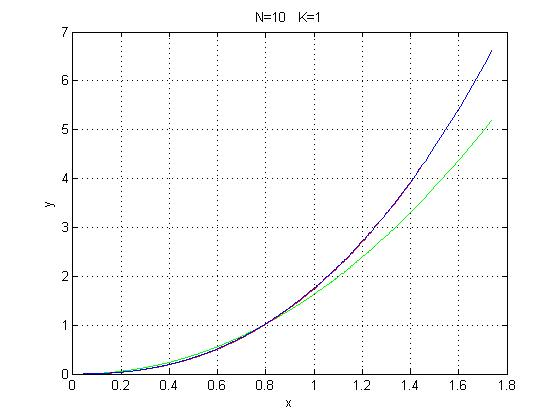
\includegraphics[width=1.0\textwidth]{k1n10.jpg} 
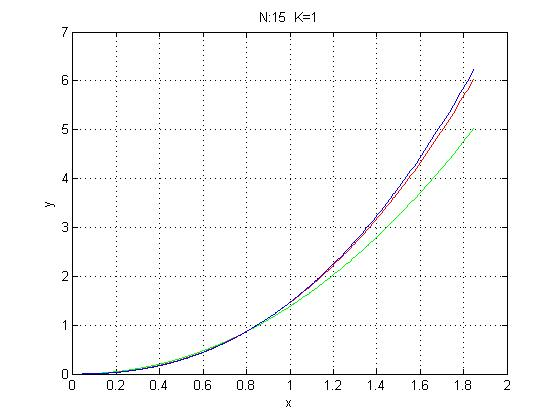
\includegraphics[width=1.0\textwidth]{../k1n15.jpg}\\
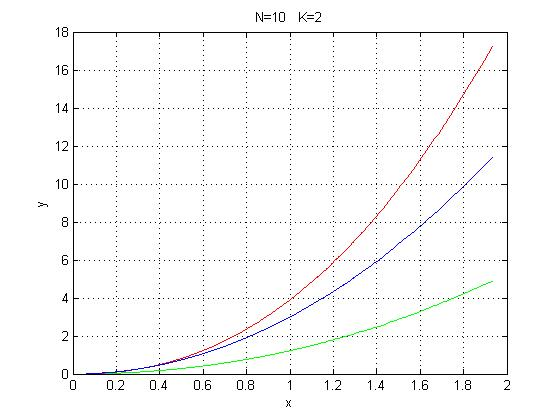
\includegraphics[width=1.0\textwidth]{../k2n10.jpg}\\
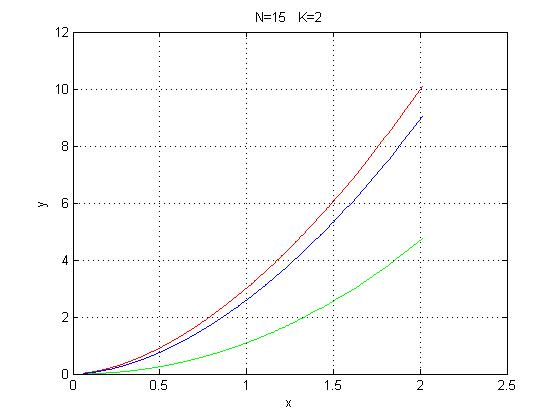
\includegraphics[width=1.0\textwidth]{../k2n15.jpg}\\
\newpage
The graphics for $\alpha=6$ and $\beta=2.5$ When the Prior parameter $(a, b )= (6, 1)$ and $(c, d) =(5, 2)$\\
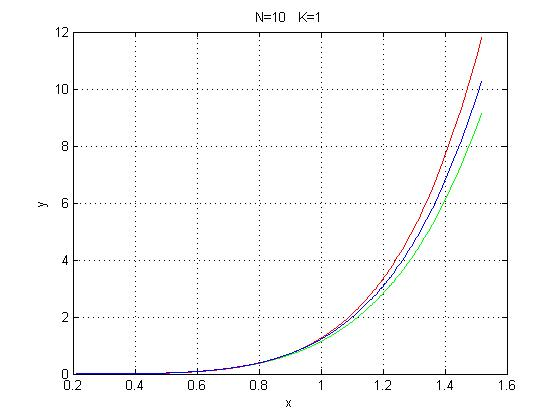
\includegraphics[width=1.0\textwidth]{n10k1a6.jpg} 
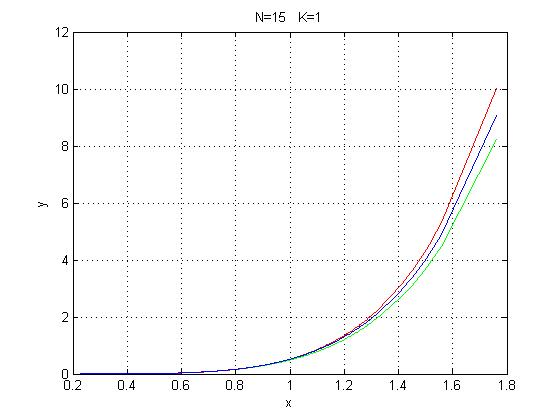
\includegraphics[width=1.0\textwidth]{../k1n15a6.jpg}\\
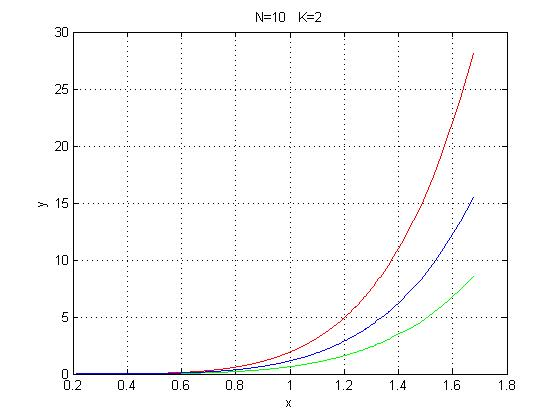
\includegraphics[width=1.0\textwidth]{../k2n10a6.jpg}\\
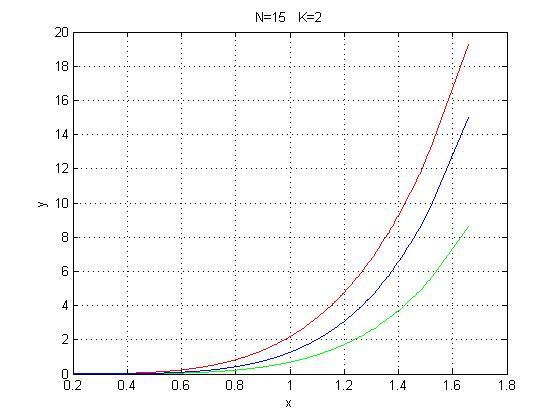
\includegraphics[width=1.0\textwidth]{../k2n15a6.jpg}\\
\newpage
\section{References}
\begin{thebibliography}{99}
\bibitem{}Ahsanullah, M. (1995). Record Statistics. Commack, New York: Nova Science Publishers, Inc.
\bibitem{}Ahsanullah, M. (1996). Generalized order statistics from two parameter uniform distribution. Commun. Statist. Theor. Meth. 25(10):2311–2318.
\bibitem{} Ahsanullah, M. (2000). Generalized order statistics from exponential distribution. J. Statist. Plann. Infer. 85:85–91.
\bibitem{}Arnold, B. C., Balakrishnan, N., Nagaraja, H. N. (1992). A First Course In Order Statistics. New York: John Wiley and Sons, Inc.
\bibitem{}Arnold, B. C., Balakrishnan, N., Nagaraja, H. N. (1998). Records. New York: John Wiley and Sons, Inc.
\bibitem{}Cramer, E., Kamps, U. (1996). Sequential order statistics and k-out-of-n systems with sequentially adjusted failure rates. Ann. Inst. Statist. Math. 48:535–549.

\bibitem{}Cramer, E., Kamps, U. (1998). Maximum likelihood estimation with different sequential k-out-of-n system. Adv. Stochastic Models Reliabil. Qual. Safety 7:101 -111.

\bibitem{}Cramer, E., Kamps, U. (2000). Relations for expectations of functions of generalized order statistics. J. Statis. Plann. Infer. 89:79–89.

\bibitem{}Cramer, E., Kamps, U. (2001). Sequential k-out-of-n systems. In: Balakrishnan, N. Rao, C. R. eds. Handbook of Statistics: Advances in Reliability. Vol. 20. ch. 12. Amsterdam: Elsevier, pp. 301–372.

\bibitem{}David, H. A. (1981). Order Statistics. 2nd ed. New York: John Wiley and Sons, Inc. Evans, I. G. Ragab, A. S. (1983). Bayesian inferences given a type 2 censored sample from Burr distribution. Commun. Statist. Theor. Meth. 12:1569–1580.

\bibitem{}D. V. Lindley, Approximate Bayesian methods, J. Trabajos de Estadistica, 31 (1980),
223-237.

\bibitem{} D. Moore and A. S. Papadopoulos, The Burr type XII distribution as a failure model under various loss functions, Microelectronics and Reliability, 40(2000), 2117-2122.

\bibitem{}D. V. Lindley, Approximate Bayesian methods, J. Trabajos de Estadistica, 31 (1980), 223-237.

\bibitem{}Kamps, U., Gather, U. (1997). Characteristic properties of generalized order statistics from exponential distributions. Applicationes Mathematicae 24(4):383–391.
\bibitem{}Mustafa Nadar and Fatih Kızılaslan (2015). Estimation and prediction of the Burr type XII distribution based on record values and inter-record times, Journal of Statistical Computation and Simulation, 85:16, 3297-3321.

\bibitem{}P. H. Liu and F. L. Chen, Process capability analysis of non-normal process data using the Burr XII distribution, International Journal of Advanced Manufacturing Technology, 27(2006), 975-984.

\bibitem{}S. J. Wu, Y. J. Chen and C. T. Chang, Statistical inference based on progressively censored samples with random removals from the Burr type XII distribution, Journal of Statistical Computation and Simulations, 77(2007), 19-27.

\bibitem{}S. K. Safi and R. H. Ahmed, Statistical estimation based on generalized order statistics from Kumaraswamy distribution, Proceeding of the 14st Applied Stochastic Models and Data Analysis (ASMDA)International Conference, Mataro (Barcelona), Spain, 25-28, (2013).

\bibitem{}Tadikamalla, P. R. (1980). A look at the Burr and related distributions. Inter. Statist. Rev. 48:337–344.

\bibitem{}Udo Kamps, A concept of generalized order statistics, Journal of Statistical Planning and Inference Volume 48, Issue 1, 1 November 1995, Pages 1–23

\bibitem{} U. Kamps, A Concept of Generalized Order Statistics, B.G. Teubner Stuttgart, (1995).

\bibitem{}Z. F. Jaheen,  Estimation Based on Generalized Order Statistics from the Burr Model, Communications in Statistics Theory and Methods, 34 (2005), 785-794.


\end{thebibliography}
\end{document}
